%
% (File) acl2018.tex
%
%% Based on the style files for ACL-2017, with some changes, which were, in turn,
%% Based on the style files for ACL-2015, with some improvements
%%  taken from the NAACL-2016 style
%% Based on the style files for ACL-2014, which were, in turn,
%% based on ACL-2013, ACL-2012, ACL-2011, ACL-2010, ACL-IJCNLP-2009,
%% EACL-2009, IJCNLP-2008...
%% Based on the style files for EACL 2006 by
%%e.agirre@ehu.es or Sergi.Balari@uab.es
%% and that of ACL 08 by Joakim Nivre and Noah Smith

\documentclass[11pt,a4paper]{article}
\usepackage[hyperref]{acl2018}
\usepackage{times}
\usepackage{latexsym}

\usepackage{color}

\usepackage{amsmath,amsthm}
\theoremstyle{definition}
\newtheorem*{defn}{Definition}

\usepackage[ruled]{algorithm2e}

\usepackage{graphicx}
\usepackage{epstopdf}


\usepackage{url}

%\aclfinalcopy % Uncomment this line for the final submission
%\def\aclpaperid{***} %  Enter the acl Paper ID here


%\setlength\titlebox{5cm}
% You can expand the titlebox if you need extra space
% to show all the authors. Please do not make the titlebox
% smaller than 5cm (the original size); we will check this
% in the camera-ready version and ask you to change it back.
\newcommand{\secref}[1]{Section \ref{#1}}
\newcommand{\figref}[1]{Figure \ref{#1}}
\newcommand{\eqnref}[1]{Eq. (\ref{#1})}
\newcommand{\exref}[1]{Example \ref{#1}}
\newcommand{\algoref}[1]{Algorithm \ref{#1}}
\newcommand{\tabref}[1]{Table \ref{#1}}
\newcommand{\socvec}{SocVec}
\newcommand{\argmin}{\operatornamewithlimits{argmin}}
\newcommand{\argmax}{\operatornamewithlimits{argmax}}
\newtheorem{example}{Example}
\newtheorem{lemma}{Lemma}
\newtheorem{definition}{Definition}
\newcommand{\cut}[1]{}

\newcommand\BibTeX{B{\sc ib}\TeX}
\newcommand{\KZ}[1]{\textcolor{red}{Kenny: #1}}
\newcommand{\KQ}[1]{\textcolor{blue}{Kangqi: #1}}
\newcommand{\YY}[1]{\textcolor{orange}{Yangyang: #1}}

\title{Triple Construction Algorithms for Joint Extraction of Entities and Relations}

\author{First Author \\
  Affiliation / Address line 1 \\
  Affiliation / Address line 2 \\
  Affiliation / Address line 3 \\
  {\tt email@domain} \\\And
  Second Author \\
  Affiliation / Address line 1 \\
  Affiliation / Address line 2 \\
  Affiliation / Address line 3 \\
  {\tt email@domain} \\}

\date{}

\begin{document}
\maketitle
\begin{abstract}
Previously a novel tagging scheme was proposed to jointly
extract entities and relations at the same time and showed
good results. In this process, relation triples must be
eventually recovered from the predicted sequence of special tags.
Previous algorithm to construct the triples was simple and naive.
This paper presents a few new triple construction algorithms
that results in substantial improvement on the end-to-end
relation extraction task.
\end{abstract}


\section{Introduction}
\label{sec:intro}

Evaluation of dialogue systems is an open problem. Existing
automatic evaluation metrics for chitchat systems are similar to those for 
other text generation tasks (e.g., machine translation \citep{papineni-etal-2002-bleu}, question-answering \citep{rajpurkar-etal-2016-squad}, 
summarization \citep{lin-2004-rouge}), which depends on calculating word 
overlaps with reference responses. 
However, for chitchats, there are usually 
many alternative but plausible responses given a situation, 
perhaps more than any other text generation task mentioned above. 
A limited number of reference responses are 
not sufficient to determine how good a generated response is. 
Moreover, such static settings are not good at
assessing an interactive, context-sensitive system.

Interactive human evaluation metrics usually 
involve a Likert scale evaluation after a multi-turn conversation 
with the bot to be assessed. 
While this method is a step up from the previous static evaluation, 
it is difficult for human judges to give a concrete score to
any bot.
%\KZ{But are we also asking judges to score invidividual bots, which is difficult?} 
Comparing the performance of two bots is easier. 
Thus ACUTE-EVAL~\citep{DBLP:journals/corr/abs-1909-03087} asks the 
judges to make a binary judgment of who is better in conversations between two identical bots 
or between a human and a bot. A more advanced version of that
is \textit{Spot The Bot}~\cite{deriu-etal-2020-spot} which models the 
human evaluation of a 
conversation after the Turing test. However, such a process is still 
time-consuming and costly, compared with automatic evaluations.

In our opinion, a good method for evaluating multi-turn 
conversational model/system 
should satisfy the following requirements:
i) be as efficient and inexpensive as possible;
ii) can truly reflect a model's ability to conduct a human conversation; 
iii) evaluation results should correlate well with human judgments;
iv) can be used to compare and rank the capabilities of a set of models/systems.
  
Toward that goal, in this work, we propose an automatic interactive evaluation 
framework, which is called \textit{ChatMatch}(CM) for chitchat
agents. This framework can be used to rank a number of bots with little
time and minimum human effort.  Above all, we want to emphasize 
the significance of direct interactions between bots 
in the evaluation.
%\textcolor{red}{Reviewer 1 said that he didn't understand this sentence. Maybe remove "the observation"?} 
People tend to believe that human-bot conversations are more reliable 
and produce more comprehensive evaluations of chatbots' capabilities. 
This is not always true. As human annotators know their counterpart is a robot, 
they tend to ask common and goal-directed questions. 
On the other hand, some bot-bot chat logs in our experiments show that, 
surprisingly, conversations between different bots may expose their strengths 
and weaknesses never seen in human-bot conversations. 
\figref{fig:two convs} gives two small chat fragments, illustrating such
differences.
While talking about hobbies, human keeps asking the bot some blunt
questions, which leads to dull responses from the bot.
However, in a bot-bot setting, two bots, including the same bot in the previous
conversation, start explaining their hobbies to each other, producing a more
interesting conversation. 

\begin{figure}[ht!]
 \centering

% \subfigure[Chat snippet between human and bot (Plato-2)]{
\subfigure[Chat snippet between human and bot]{ 
 %  \centering
  %  \begin{minipage}[t]{0.5\linewidth}
  \includegraphics[width=0.95\linewidth]{eg4.eps}\label{fig:sub-first}
  %  \end{minipage}
 }
 
 \subfigure[Chat snippet between two bots]{
  % \centering
  % \begin{minipage}[t]{0.5\linewidth}
  \includegraphics[width=0.95\linewidth]{figs.eps}\label{fig:sub-second}
  % \end{minipage}
 }
 \caption{Snippets from human-bot and bot-bot chat logs}
\label{fig:two convs}
\end{figure}

Our framework consists of two components: \textit{competition} and 
\textit{scoring}, which interoperate with each other. 
The competition is modeled
after most sports tournaments such as soccer or ping pong. 
There are three levels of competitions. From bottom up, they are:
game-level, match-level and tournament-level. 
Each match consists of several games. During a game, two bots will converse 
freely with each other and a virtual judge will score their performances 
according to a set of user-defined criteria such as consistency and fluency, 
etc.  These criteria are flexible and extensible.
%As an example like \figref{fig:example} shows, 
%Bot $A$ will be 
%penalized twice for repeating while Bot $B$ will be penalized once for 
%contradicting itself. In addition to the penalty, 
%a bonus point is rewarded to $A$
%who shows to produce relevant response with long term memory. 
%\KZ{Do we still have this as a criterion?}
%However, the specific bonus and penalty settings may vary 
%depending on the domain and scenarios that the experiment is 
%set in. 

%\begin{figure}[th!]
%	\centering
%	\includegraphics[width=0.95\columnwidth]{example.eps}
%	\caption{A chat snippet between two bots.}
%	\label{fig:example}
%\end{figure}

The main contributions of this paper are:
\begin{itemize}
\item We propose the first interactive evaluation framework for chatbots which
is based solely on bot-bot conversations and modeled after sports competitions (\secref{sec:competition}).
\item We designed three algorithms to score \textit{diversity}, \textit{consistency}, \textit{relevance}, three important dimensions in a bot's chatting 
abilities.
\item  The entire scoring process is fully automated and efficient. 
In our experiments, the system can rank seven bots in less than 
three minutes on average (\secref{sec:scoring}, \secref{sec:time}).
\item  Our experiments show that the results produced by our framework
closely correlate with the human evaluation results. 
Results also show that our framework outperforms 
several recent strong baseline evaluation systems (\secref{sec:main}).
%\item %We demonstrate the improvements in efficiency 
%using direct chat logs between bots.
%\KZ{Maybe this should not be a contribution but part of the conclusion?}
%We show that the chats between bots are impressively informative, 
%even richer than the chats between humans and bots.
%This suggests some possible directions to improve 
%the capabilities of bots in the future.
%(e.g., by having them learn from each other)  (\secref{sec:diversity})
\end{itemize}

%\section{E-commerce Concept Net} 
\label{sec:ecn}

%A user need is a motive that prompts a user to buy a product or service.
In our e-commerce concept net \footnote{This section only gives
a brief introduction of the E-commerce Concept Net, while more details will be 
discussed in a separate paper.},
user needs are conceptualized as various shopping scenarios, also known as ``concepts''.
%In order to cover as many user needs as possible,
%a thorough analysis on query logs, product titles and open-domain text from web is conducted .
%Based on years of experience in e-commerce,
Each concept can be expressed using values drawn from $8$ different domains of
an ``e-commerce concept vocabulary'', which is shown in \figref{fig:kg} (b).
%\KZ{I think the concept ontology should be renamed to ``concept vocabulary''. Ontology
%means the knowledge graph itself. So this naming maybe confusing.}
For example, ``Outdoor Barbecue'' can be written as 
``\textit{Location}: outdoor, \textit{Incident}: barbecue'', 
and ``Breakfast for Pregnancy'' can be written as ``\textit{Object}: pregnant women, \textit{Cate/Brand}: breakfast''.
Concepts are then related to their representative items, categories, brands respectively, to form the complete e-commerce concept net.
%\KZ{What do you mean by ``other concepts''? These are not from the concept
%ontology right? A bit confusing here.} 
It should be noticed that there is a hierarchy within each domain. For example, ``Shanghai'' is a city in ``China'' in the domain of \textit{Location} and ``pregnancy'' is a special stage of a ``woman'' in the domain of \textit{Object}.  Vocabulary terms at different levels can be combined and result in different concepts.
Accordingly, those concepts are naturally related to form a hierarchy as well.
%\noindent
%\textbf{1) Time}: seasons, holidays, any time related terms;

%\noindent
%\textbf{2) Location}: countries, cities, any space related terms;

%\noindent
%\textbf{3) Object}: group of human beings (man/woman/olds/kids...), animals, plants, etc;

%\noindent
%\textbf{4) Function}: terms describe a functional use of product, such as keeping you warm, making you slim, etc;

%\noindent
%\textbf{5) Incident}: activities such as barbecue, hiking, fishing and other actions;

%\noindent
%\textbf{6) Category/Brand}: categories and brands in general e-commerce knowledge graph;

%\noindent
%\textbf{7) Style}: style words, usually describing categories and brands;

%\noindent
%\textbf{8) IP}: intellect properties such as a famous sports star, song or movie.

%\noindent
%Examples of each domain's vocabulary are shown in . 

Besides the vocabularies to describe concepts, there are constraints to each concept. 
The aspects of concept \textit{schema} include
 \textit{gender}, \textit{life stage} \footnote{Life stage is divided into: pregnancy, infant, kindergarten, primary school, middle school and high school in Taobao.}, etc.
which actually corresponds to user profile.
For example, the schema of ``Breakfast for Pregnancy'' will be ``\textit{gender}: female, \textit{life stage}: pregnancy'', which indicates the group of users who are most likely to need this concept.

\begin{table}[th]
	\centering
	\small
	\begin{tabular}{|l|r|r|r|r|}
		\hline
		\multirow{4}{*}{Ontology Vocab.} 
		&\# Time &\# Location &\# Object &\# Func.  \\
		\cline{2-5}
		& 127 & 7,052 & 247 & 3,693 \\
		\cline{2-5}
		&\# Inci. & \# Cate/Bra. & \# Style &\# IP  \\
		\cline{2-5}
		& 9,884 & 44,860 & 1,182 & 21,230 \\
		\hline
		\# Concepts (Raw) & \multicolumn{1}{c|}{35,211} &
		\multicolumn{2}{c|}{\# Concepts (Online)} & \multicolumn{1}{c|}{7,461} \\ 
		\hline
		\# Items & \multicolumn{1}{c|}{1 billion} &
		\multicolumn{2}{c|}{\# Categories/Brands} & \multicolumn{1}{c|}{19K/5.5M} \\ 
		\hline
		%		\bottomrule
	\end{tabular}
	\caption{Statistics of E-commerce Concept Net.}
	\label{tab:data}
\end{table}


%Crowdsourcing effort is important during the construction of e-commerce concept net, 
%aiming to make sure the overall quality fits the requirements of industry applications. 
%All the concepts and edges generated automatically will be randomly sampled in batches to test accuracy, 
%and only those batches pass the test will be added into the graph.
\tabref{tab:data} shows the statistics of the concept net used in this
paper~\footnote{Preview of concept data can be found at \url{https://github.com/angrymidiao/concept_net}.}.
There are 35,211 concepts in total at current stage, 
among which 7,461 concepts are already deployed in our online recommender system, covering over 90\% categories of Taobao and each concept is related with 10.4 categories on average.

\section{Problem}
\label{sec:problem}

In this section, we formally define the problem of user needs inference.
Let $\bi{U}$, $\bi{V}$ denote the sets of users, items respectively.
The inputs of our problem are as follows:

\noindent
\textbf{1) User behavior on items}. For each $u\in \bi{U}$,  a behavior sequence 
$b= \{b_1, b_2, \cdots, b_n\}$ is a list of behaviors in time order, 
where $b_i$ is the $i^{th}$ behavior and $b_n$ is the latest one. 
Each user behavior contains a user-item interaction, 
detailed as $b_i = <v_i, type_i, time_i>$, where $v_i \in \bi{V}$, 
$type_i$ is the type of behavior, such as click or purchase, and
$time_i$ denotes the specific time of the behavior.

\noindent
\textbf{2) E-commerce concept net}. Concept net $\bi{G}$ consists of massive triples $(h, r, t)$, 
where $h, t\in \bi{E}$, $r\in \bi{R}$ denote the head, tail and relation.
$\bi{E}$ and $\bi{R}$ are entities and relations in the concept net.
While most items in $\bi{V}$ can be linked to entities in $\bi{E}$, 
some items may not, since the item pool in e-commerce platforms changes frequently. 
The set of all concepts in $\bi{G}$ is denoted as $\bi{C}$.

\noindent
\textbf{3) Side information}. 
For each user $u\in \bi{U}$, we have corresponding profile information $h$, 
such as \textit{gender}, \textit{kid's life stage} and long-term preferred categories, etc.
For each concept $c\in \bi{C}$, we have its schema $s$ introduced in \secref{sec:ecn};


Given above inputs, the goal of user needs inference is to predict potential need in concept $c$ for each user $u$. We aim to learn a prediction function $\hat y_{uc} = \bi{F}(u, c; \theta)$, denoting the probability concept $c$ is needed by user $u$, and $\theta$ is the model parameters.


%\section{Joint RE Tagging Model}
\label{sec:tagging}

We propose a joint learning model with three modules, namely
sentence representation, RTD and the basic RE tagging, 
as illustrated in \figref{fig:model}. 
Sentence representation module is to encode a sentence to a matrix, which is the 
base of whole model. Other two modules deal with the auxiliary task and 
the main task. Note that superscript ($^S$), ($^R$) and ($^T$) is used
to indicate variables belonging to sentence representation,
RTD and basic RE tagging modules respectively.


\begin{figure}[th]
\centering
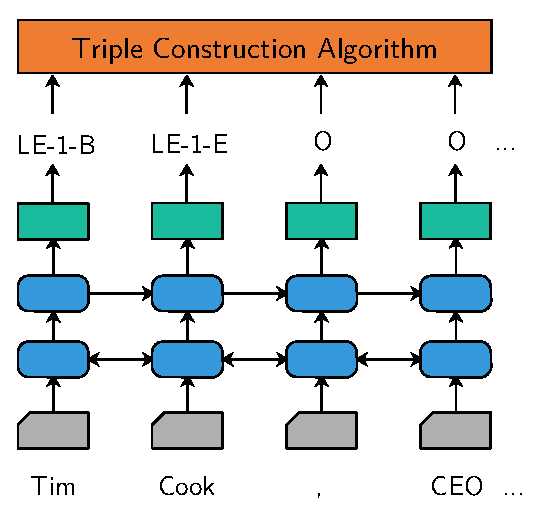
\includegraphics[width=\columnwidth]{pictures/model.eps}
\caption{The joint RE tagging model \label{fig:model}}
\end{figure}

\subsection{Sentence Representation Module}
Sentence representation module represents token sequence and extracts low level
features. A sentence $s$ is a sequence of tokens $(w_1, w_2, \ldots, w_i,
\ldots, w_n)$, where $w_i$ is the $i^{th}$ token in $s$, and is represented by
a 1-hot vector $v_i$ with length $|\mathcal{V}|$, where $\mathcal{V}$ is 
the vocabulary. We pretrain word embedding matrix $D$, and use a BiLSTM to
represent a sentence:

\begin{align*}
    \overrightarrow{h}_i^S &= LSTM(\overrightarrow{h}_{i-1}^S, v_iD) \nonumber \\
    \overleftarrow{h}_i^S &= LSTM(\overleftarrow{h}_{i+1}^S, v_iD) \nonumber \\
    h_i^S &= [\overrightarrow{h}_i^S, \overleftarrow{h}_i^S] \nonumber
\end{align*}

Where $\overrightarrow{h}_i^S$ and $\overleftarrow{h}_i^S$ are the hidden state
of forward and backward LSTM. Their concatenation $h_i^S$ is used as the feature
of token $w_i$.


%\subsection{NER Module}
%Typically, NER can also be treated as Tagging problem under ``BIES'' tagging
%scheme \YY{Add some references}. For example, tag sequence ``Person-B Person-E''
%of ``Tim Cook'' indicate that this is a person entity which begins with ``Tim''
%and ends with ``Cook''.
%
%
%
%We decode entity tag sequence using another LSTM. For token
%$w_i$, the input of decoder LSTM, $h_i^S$, is from the sentence module, and the
%output is $h_i^E$. Formally,
%
%\begin{align*}
%  h_i^E &= LSTM(h_{i-1}^E, h_i^S) \nonumber \\
%  p_i^E &= softmax(W^Eh_i^E + b^E) \nonumber
%\end{align*}
%
%$p_i^E$ is the probability vector over NER tag set. Given entity tag sequence,
%all entities can be recovered easily without ambiguity. \YY{Add references}
%
%

\subsection{RTD Module}
The RTD sub-task is similar to RC but detects all relation types in a sentence
without entity information. Different from tagging problem which predicts each
tag on the feature representation of each token, relation type is bounded with
the semantic of whole sentence. We use a CNN to make this multi-label
prediction.

The input of CNN is a feature matrix $H^S$ from sentence module, each column is
the feature vector of corresponding token. Therefore, $H^S$ has two dimension, feature
dimension and sentence length dimension. Considering the linear structural of
sequence, here we choose 1d convolution by treating the feature dimension as
input channels. We
use $K$ kernels to extract sentence level features. The output of $j$th kernel
is $conv_j$. Then max pooling is applied  get the maximum feature value
$pool_j$. The representation of whole sentence $h^R$ is the combination of
$pool_j$ of each kernel. The size of feature vector $h^R$ is the number of
kerners $K$. Here, we can treat each kernel as a feature extractor which is
responsible for some kind of sentence level feature.

\begin{align*}
  H^s &= [h_1^S; h_2^S; \ldots; h_n^S] \nonumber \\
  conv_j &= Relu(kernel_j(H^S)) \nonumber \\
  pool_j^R &= \max(conv_j) \nonumber \\
  h^R &= [pool_1^R, pool_2^R, \ldots, pool_K^R] \nonumber \\
  p_i^R &= sigmoid(W^RH^R + b^R) \nonumber
\end{align*}

To predict relation types, We use a linear layer to convert $h^R$ to label space
vector. Because RTD is a multi-label classification problem, sigmoid function is
chosen as activation function. 
The $k$th element of sigmoid output $p_i^R$ is the
probability of $k$th relation type mentioned in the sentence or not.

\KZ{Add a sentence or two to highlight high level feature fed to
the basic tagging module.}

\subsection{Basic RE Tagging Module}

We use a LSTM to decode the RE tags. The input for 
token $w_i$ is  $h_i^S$ from sentence module, and the output is $h_i^T$. 
$h_i^T$ is a feature representation of token $w_i$, which extracts features by
focusing on the tokens near $w_i$. 
We argue that relation extraction should be based on 
both local and global features. Local features means the
information near by one token while global features means the information of
whole sentence. Obviously, for token $w_i$, the local features can be
represented by $h_i^T$. We use the output $h^R$ of max pooling in the RTD module
as global features, which is a feature representation of the sentence from 
the angle of relation semantic information. 
We call the concatenation of the local features
$h_i^T$ and global features $h^R$,  $h_i^{TR}$, which is used to
predict the tag of $w_i$. Intuitively, mixed features add capabilities to
the decoder. Before predicting the tag by the local features, the decoder can
have a glance at the relation information of the whole sentence. Formally,

\begin{align*}
  h_i^T, c_i^T &= LSTM(h_{i-1}^T, c_{i-1}^T, h_i^S) \nonumber \\
  h_i^{TR} &= [h_i^T, h^R] \nonumber \\
  p_i^T &= softmax(W^Th_i^{TR} + b^T) \nonumber
\end{align*}


%\section{Model Training}
\label{sec:train}

There are two tasks in our joint model. We need one loss function for each 
task to train the joint model. We use a weighted sum of these losses as
the joint loss.

%\subsection{NER Tagging Loss}
%As for NER module, we maximize the log-probability of correct tags. Given a
%sentence, most of tokens do not take part in any entities, they share the same
%tag ``O'' while only a few tokens take part in some entities. Obviously, this
%is a unbalance classification problem. Therefore, we weight the loss for
%different tags.
%
%
%\begin{equation}
%  \begin{aligned}
%    L^E = \frac{1}{M} \max{
%      \sum_m^M{
%        \sum_i^N{
%          \log(p_{i, k_{\hat{e}}}^E) \cdot I^E(\hat{e}),
%        }
%      }
%    } \nonumber
%  \end{aligned}
%\end{equation}
%where $M$ is the size of the corpus. $N$ is the length of sentence.
%$\hat{e}$ is the correct tag of token $w_i$, and $k_{\hat{e}}$ is the index of
%tag $\hat{e}$ is the tag set. $p_{i, k_{\hat{e}}}$ is the probability value of the
%correct tag $\hat{e}$. $I^e(e)$ is the loss weight function which is defined as
%follows:
%
%\begin{equation}
%  \begin{aligned}
%    I^E(e) =
%    \begin{cases}
%      1,        & if \  e = \text{'O'} \\
%      \alpha_e, & if \  e \neq \text{'O'}, \\
%    \end{cases} \nonumber
%  \end{aligned}
%\end{equation}
%where $\alpha_e$ is the loss weight of entity tag. The loss weight of tag ``O'' is constant
%$1$.
%

\subsection{RTD Loss}
In the RTD module, we max the log probability of correct relation label. Because
most of sentence does not mention even one relation type, this is a unbalance
multi-label classification problem. We also weight the loss function.

\begin{align*}
  L^R = \frac{1}{M} \max &\sum_m^M\sum_i^N
  \biggl[ \hat{r}_i \log(p_i^R) \cdot I^R(\hat{r}_i) + \\
  &{} (1 - \hat{r}_i) \log(1 - p_i^R) \cdot I^R(\hat{r}_i)
    \biggr],
\end{align*}
where $\hat{y}_i$ is the correct relation type vector. $p_i^R$ is the predicted
probability vector. $I^R(r)$ is the loss weight function which is defined as
follows:

\begin{equation}
  \begin{aligned}
    I^R(r) =
    \begin{cases}
      1,        & if \  r = 0 \\
      \alpha_r, & if \  r = 1 \\
    \end{cases} \nonumber
  \end{aligned}
\end{equation}
where $\alpha_r$ is the weight of mentioned relation type. For all unmentioned type,
the weight is 1.

\subsection{Basic RE Tagging Loss}
For end-to-end RE module, we max the probability of correct relation tag in the
same way as NER module.

\begin{equation}
  \begin{aligned}
    L^T = \max{
      \sum_m^M{
        \sum_i^N{
            \log(p_{i, k_{\hat{t}}}^T) \cdot I^T(\hat{t}),
        }
      }
    } \nonumber
  \end{aligned}
\end{equation}
where $\hat{t}$ is the correct tag of token $w_i$. $k_{\hat{t}}$ is the index of
$\hat{t}$ in the tag set. Due to $p_i$ is the probability vector of token $w_i$
over tag set, $p_{i, k_{\hat{t}}}^T$ is the probability of the correct tag of
$w_i$. $I^T(t)$ is loss weight function which is defined as follows:

\begin{equation}
  \begin{aligned}
    I^T(t) =
    \begin{cases}
      1,        & if \  t = \text{'O'} \\
      \alpha_t, & if \  t \neq \text{'O'}, \\
    \end{cases} \nonumber
  \end{aligned}
\end{equation}
where $\alpha_t$ is the loss weight of relation tag. The loss weight of tag ``O'' is
constant $1$.

%\subsection{Joint Loss}
%We use the weighted sum of these 3 loss as joint loss.
%\begin{equation}
%  \begin{aligned}
%    L = \lambda_eL^E + \lambda_rL^R + \lambda_tL^T, \nonumber
%  \end{aligned}
%\end{equation}
%where $\lambda_e$, $\lambda_r$ and $\lambda_t$ are weight values of 
%3 tasks respectively. The larger weight value is, 
%the bigger impact of the task on the shared parameters.
%



\section{Relation Triple Construction}
\label{sec:triple}

In this section, we introduce triple construction algorithms for
converting tagging sequences into relation triples.
Refer to \figref{fig:intro}, the tag of each word contains 
both named entity and relation type information.
Given a specific relation type $r$, we extract all
different $e_1$ and $e_2$ entities associated with $r$ from a tagging sequence,
and the algorithm recognizes all entities to be paired, and produce ($e_1$, $r$, $e_2$) results.
This construction step is not trivial,
because the input sequence could be long and contain multiple entities.
%which is not a trivial step, because the input sequences could be long,
%and many entities can be extracted within one sentence.

In this case, we attempt a group of construction algorithms.
The framework of these algorithms is described in \algoref{algo:construct}.
Given a tag sequence and a relation type $r$,
the algorithm first collects all associated entities $e_1$ and $e_2$ into lists $E_1$ and $E_2$,
then picks one $e_1$ and $e_2$ from the list by greedy strategy,
combining a new triple ($e_1$, $r$, $e_2$),
and removes the two entities from the corresponding list.
The picking process runs repeatly, until no more entity pairs can be combined.
In the following part of the section, We present \textit{random} picking algorithm,
the \textit{$e_1$-First} and \textit{$e_2$-First} algorithm which focus on dominating entities of a triple,
the \textit{Distance-First} and \textit{Order-First} algorithm
leveraging distance and sequential features between the extracted entities.
In which, Order-First was proposed by Zheng et al.~\shortcite{Zheng2017}.
%The last one was proposed by \cite{Zheng2017}.

%Given the RE tagging sequence, triple construction algorithm
%detects tagged entities belonging to each target relation type $r$,
%and pick the most possible combinations ($e_1$, $e_2$) from them.
%The combination strategy is not trivial, since there may be
%serveral $e_1$s and $e_2$s sharing the same relation type.
%We present 4 different construction algorithms,
%$e_1$-First, $e_2$-First, Distance-First, and Order-First.
%%to construct relation triple from RE tag sequence.
%The last one was proposed by \cite{Zheng2017}.




%Given relation tag sequence, all the predicted $e_1$ and $e_2$ can be abtained
%easily without ambiguity. There may be several $e_1$s and
%$e_2$s which share same relation type. Triple constraction algorithm is
%responsible to choose the most possible entity pair ($e_1$, $e_2$) under same
%relation type.


\begin{algorithm}%[H]
  \small
  \caption{Framework of Triple Construction Algorithm}
  \label{algo:construct}
  \SetKwInOut{Input}{input}
  \SetKwInOut{Output}{output}
    
  \Input{Relation tag sequence $TS$ of one sentence}
  \Output{Relation triples $RT$}
  
    \BlankLine
    \For{each mentioned $r$}{
      $E_1 \leftarrow$ all $e_1$ belonging to $r$ from $TS$ \;
      $E_2 \leftarrow$ all $e_2$ belonging to $r$ from $TS$ \;
      \While{both $E_1$ and $E_2$ are not empty}{
        $e_1, e_2 \leftarrow$ $greedy\_picking$($E_1, E_2$) \;  
        %$e_1 \leftarrow$ random sample an $e_1$ from $E_1$ \;
        %$e_2 \leftarrow$ random sample an $e_2$ from $E_2$ \;
        add ($e_1$, $r$, $e_2$) to $RT$ \;
        remove $e_1$ from $E_1$ \;
        remove $e_2$ from $E_2$ \;
      }
    }
\end{algorithm}



\subsection*{Random Construction Algorithm}
The random strategy is regarded as the baseline of all construction algorithms.
For each pass, the algorithm randomly picks one $e_1$ from $E_1$, and one $e_2$ from $E_2$,
then construct the ($e_1$, $r$, $e_2$) triple.

%In a sentence, for all $e_1$s and $e_2$s sharing the same relation type $r$,
%we randomly choose an $e_1$ and an $e_2$ to construct a triple ($e_1$, $r$,
%$e_2$). This algorithm can be treat as the baseline of all construction algorithms.


%\begin{algorithm}%[H]
%  \small
%    \caption{Random}
%    \label{algo:rand}
%    \SetKwInOut{Input}{input}
%    \SetKwInOut{Output}{output}
%    
%    \Input{Triple tag sequence $TS$ of one sentence}
%    \Output{Relation triples $RT$}
%  
%    \BlankLine
%    \For{each mentioned $r$}{
%      $E_1 \leftarrow$ all $e_1$ belonging to $r$ from $TS$ \;
%      $E_2 \leftarrow$ all $e_2$ belonging to $r$ from $TS$ \;
%      \While{both $E_1$ and $E_2$ are not empty}{
%        $e_1 \leftarrow$ random sample an $e_1$ from $E_1$ \;
%        $e_2 \leftarrow$ random sample an $e_2$ from $E_2$ \;
%        add ($e_1$, $r$, $e_2$) to $RT$ \;
%        remove $e_1$ from $E_1$ \;
%        remove $e_2$ from $E_2$ \;
%      }
%    }
%\end{algorithm}



\subsection*{$e_1$-First and $e_2$-First Construction Algorithms}
%Given a relation type $r$, let $E_1$ and $E_2$ denote the
%set of entities $e_1$ and $e_2$ to be paired, belonging to $r$.
%As described in \algoref{algo:e1},
$e_1$-First algorithm regards $e_1$ as the dominating entity of a triple.
For each pass, the algorithm picks the leftmost $e_1$ from $E_1$,
and then pick the nearest
\footnote{The distance of two entities is defined as the number of words
between them in the tagging sequence.}
$e_2$ in $E_2$.
%pairing with the nearest $e_2$ in $E_2$,
%then remove both $e_1$ and $e_2$ from the corresponding sets.
%The picking process runs iteratively, until no more entity pairs can be combined.
%
%$e_1$-First treats $e_1$ of a triple as the dominating entity. For
%a tag sequence, $e_1$-First algorithm goes through it
%from left to right, for each predicted $e_1$ with type $r$, find the
%nearest $e_2$ with the same type $r$. This entity pair will be constructed as a
%triple \{$e_1$, $r$, $e_2$\}. See Algorithm \ref{algo:e1} for details.
%
%\begin{algorithm}%[H]
%  \small
%  \caption{$e_1$-First}
%  \label{algo:e1}
%  \SetKwInOut{Input}{input}
%  \SetKwInOut{Output}{output}
%    
%  \Input{Triple tag sequence $TS$ of one sentence}
%  \Output{Relation triples $RT$}
%  
%  \BlankLine
%  
%  \For{each mentioned $r$}{
%    $E_1 \leftarrow$ all $e_1$ belonging to $r$ from $TS$ \;
%    $E_2 \leftarrow$ all $e_2$ belonging to $r$ from $TS$ \;
%    \For{each $e_1$ in $E_1$}{
%      find the $e_2$ in $E_2$ which is nearest to $e_1$ \;
%      remove $e_2$ from $E_2$ \;
%    }
%  }
%\end{algorithm}
$e_2$-First algorithm is the exact opposite of $e_1$-First, 
where the algorithm always pick the leftmost $e_2$, and pair it with the nearest $e_1$.
%where $e_2$ of a triple is the dominating entity. For each $e_2$, it is paired with the
%nearest $e_1$ which shares same relation type with $e_2$.

\subsection*{Distance-First Construction Algorithm}
%Similar with $e_1/e_2$-First algorithms, Distance-First algorithm
%collects $E_1$ and $E_2$, then iteratively select entity pairs from them.
%The main difference is that, 
Different from previous algorithms, Distance-First algorithm treats $e_1$ and $e_2$ equally.
For each pass, the algorithm picks the nearest ($e_1$, $e_2$) pair from $E_1 \times E_2$ combinations.
%it always pick the nearest ($e_1$, $e_2$) pair
%and combine them into a new relation triple.
%Details are shown in \algoref{algo:dist}.

%It goes through the relation tag sequence several times, for each pass it
%chooses the nearest entity pair and construct a triple. Then these used entities
%will delete before next pass.

%\begin{algorithm}%[H]
%  \small
%  \caption{Distance-First} \label{algo:dist}
%  \SetKwInOut{Input}{input}
%  \SetKwInOut{Output}{output}
%  
%  \Input{Triple tag sequence $TS$ of one sentence}
%  \Output{Relation triples $RT$}
%  
%  \BlankLine
%  \For{each mentioned $r$}{
%    $E_1 \leftarrow$ all $e_1$ belonging to $r$ from $TS$ \;
%    $E_2 \leftarrow$ all $e_2$ belonging to $r$ from $TS$ \;
%    \While{both $E_1$ and $E_2$ are not empty}{
%      find the nearest ($e_1$, $e_2$) $\in E_1 \times E_2$ \;
%      add ($e_1$, $r$, $e_2$) to $RT$ \;
%      remove $e_1$ from $E_1$ \;
%      remove $e_2$ from $E_2$ \;
%    }
%  }
%\end{algorithm}

\subsection*{Order-First Construction Algorithm}
In Order-First algorithm
\footnote{The code released by Zheng shows their algorithm concretely:
https://github.com/zsctju/triplets-extraction},
$e_1$ and $e_2$ are also equally treated.
For each pass, the algorithm simply picks the leftmost $e_1$ and $e_2$ from both entity lists.
In other words, the order of both $e_1$ and $e_2$ dominate the construction results.

%The algorithm first sort $E_1$ and $E_2$ by the position of entities,
%and simply align ($e_1$, $e_2$) pairs in sequential order.
%From left to right, the first $e_1$ with
%type $r$ will pair with the first encountered $e_2$ with the same type.
%The second $e_1$ will pair with second $e_2$ with the same type and so on.
%In other words, the order of both $e_1$s and $e_2$s dominate the construction results.
%More details are in Algorithm \ref{algo:order}. 

%\begin{algorithm}%[H]
%  \small
%    \caption{Order-First}
%    \label{algo:order}
%    \SetKwInOut{Input}{input}
%    \SetKwInOut{Output}{output}
%    
%    \Input{Triple tag sequence $TS$ of one sentence}
%    \Output{Relation triples $RT$}
%  
%    \BlankLine
%    \For{each mentioned $r$}{
%      $E_1 \leftarrow$ all $e_1$ belonging to $r$ from $TS$ \;
%      $E_2 \leftarrow$ all $e_2$ belonging to $r$ from $TS$ \;
%      \While{both $E_1$ and $E_2$ are not empty}{
%        $e_1 \leftarrow$ head entity in $E_1$ \;
%        $e_2 \leftarrow$ head entity in $E_2$ \;
%        add ($e_1$, $r$, $e_2$) to $RT$ \;
%        remove $e_1$ from $E_1$ \;
%        remove $e_2$ from $E_2$ \;
%      }
%    }
%\end{algorithm}





\section{Experiment Evaluation}
\label{sec:experiment}
In this section, we first give some statistics of our corpus and evaluate the quality and quantity of the learned rules. Then, we compare with other causal knowledge bases. Next, we analyze and discuss some main sub-modules in the rule learning framework. Finally, a practical application of futures price prediction and demonstration are introduced. Our experiments are implemented in Python and SWI-Prolog\footnote{ \url{ http://www.swi-prolog.org/}}.
% and run on a computer with Intel Xeon 32 CPU(2.60GHz) and 173GB memory.
	
\subsection{Dataset}
We crawled the text dataset from Chinese financial news website \footnote{\url{ http://finance.sina.com.cn}}. The news data containing 4,991,000 articles, from 2000/7/20 to 2017/12/31, is used to rule learning.
%	, which are split into \textbf{111,330,205} sentences. The number of unique sentences is \textbf{75,572,053}, covering  \textbf{67.88\%} of the total sentences. 
The number of sentences with causal cue words is 7,147,141, accounting for 9.46\% of the total number of de-duplicated sentences (75,572,053. The repetition rate of sentences is about 32\%).
It shows that about  \textbf{14.2\%} (9.64\%/(1-32\%)) sentences explicitly express causality in online financial news sentences.
The news data containing 270,562 articles, from 2018/1/1 to 2018/11/2, is used to evaluate our framework. We set $\alpha$ to 0.5 to achieve an equal balance between generalization and specialization in rule induction. 
We set $\gamma$ to 0.3 to control the Prolog engine to reason around two steps, since more than two steps lead to obviously unreasonable results.

%	\begin{table}[]
%		\caption{Dataset Information}
%		\begin{center}
%		\begin{tabular}{|l|l|l|}
%			\hline
%			Dataset       & Train & Test \\ \hline
%			Time Interval &       &      \\ \hline
%			Number        &       &      \\ \hline
%		\end{tabular}
%	\end{center}
%	\end{table}

\subsection{Rule Evaluation}
We evaluate these rules both quantitatively and qualitatively.
\paragraph{Quantitative Evaluation}
The number of the final rules we learned is \textbf{50000}. We divide the rule quality into three levels: good, fair and bad. According to the ranking of rule confidence, we randomly select 200 rules from the top 10000 rules and manually divide them into three levels. The `good', `fair', and `bad' levels of them account for \textbf{32.5\%}, \textbf{39.0\%} and \textbf{28.5\%}, respectively.
%	\begin{table}[]
%		\centering
%		\begin{tabular}{|l|l|l|} \hline
%		 good & fair &bad \\ \hline
%			65/200(32.5\%)& 78/200(39.0\%) & 57/200(28.5\%) \\ \hline
%		\end{tabular}
%		\caption{Rule Quality}
%		\label{tab:rule_quality}
%	\end{table}

\paragraph{Qualitative Evaluation}
%\begin{align*}
%%	good
%%	{"c": ["过剩_1", "X_燃料", "产量", "", ""], "e": ["下降_1", "X_自然资源", "价格", "", ""], "relation": [["c_sc", "e_sc", "madeof"]], "ctx": {"senids": [1975666], "pattern_ids": [8]}, "ruleid": 5131, "confidence": 0.5657637042081998}
%&\text{1 (X, '产量/yield', '过剩/surplus', '', ''):-(Y, '价格/price', '下降/fall',} \nonumber\\
%&\text{'',''), IsA(X, '燃料/fuel'), IsA(Y, '自然资源/natural resource'),} \nonumber\\
%&\text{madeof(X, Y)} \\
%%{"c": ["结束_1", "X_国家", "罢工", "", ""], "e": ["下降_1", "X_金属", "价格", "", ""], "relation": [["e_sc", "c_sc", "atlocation"]], "ctx": {"senids": [341012], "pattern_ids": [6]}, "ruleid": 11607, "confidence": 0.5824045924950126}
%&\text{2 (X, '罢工/strike', '结束/stop', '', ''):-(Y, '价格/price', '下降/fall', }\nonumber\\
%&\text{'',''), IsA(X, '国家/nation'), IsA(Y, '金属/metal')}\nonumber\\
%&\text{, atlocation(Y, X)}	 \\
%%{"c": ["下降_1", "X_作物", "价格", "", ""], "e": ["减少_1", "", "", "X_作物", "面积"], "relation": [["c_sc", "e_oc", "=="]], "ctx": {"senids": [961411], "pattern_ids": [8]}, "ruleid": 978, "confidence": 0.5876590112986869}
%&\text{3 (X, '价格/price', '下降/fall', '', ''):-(X, '面积/area', '减少/fall', }\nonumber\\
%&\text{'',''), IsA(X, '作物/crop')} \\
%%fair
%%2{"c": ["下降_1", "X_国家", "储蓄率", "", ""], "e": ["下降_1", "X_国家", "增长率", "", ""], "relation": [["c_sc", "e_sc", "=="]], "ctx": {"senids": [1640122], "pattern_ids": [5]}, "ruleid": 213, "confidence": 0.7185889172176277}
%&\text{4 (X, '储蓄率/saving rate', '下降/fall', '', ''):-(X, '增长率/growth rate', }\nonumber\\
%&\text{'下降/fall','',''), IsA(X, '国家/nation')} \\
%%2{"c": ["下降_1", "", "X_产品", "", ""], "e": ["适合_1", "", "X_作物", "", ""], "relation": [["c_s", "e_s", "madeof"]], "ctx": {"senids": [1791763], "pattern_ids": [6]}, "ruleid": 19783, "confidence": 0.5634539402859007}
%&\text{5 ('', X, '下降/fall', '', ''):-('', Y, '适合/fit', '', ''), IsA(X, }\nonumber\\
%&\text{'产品/product'), IsA(Y, '作物/crop'), madeof(X, Y)}   \\
%%bad
%%1{"c": ["减少_1", "", "X_国家", "X_自然资源", "依赖性"], "e": ["增加_1", "", "", "X_燃料", "销量"], "relation": [["e_oc", "c_oc", "madeof"]], "ctx": {"senids": [1707156], "pattern_ids": [8]}, "ruleid": 4468, "confidence": 0.5717182258485046}
%%另一方面,由于日本、韩国和中国减少对中东地区进口原油的依赖性,道达尔公司希望增加对这三个国家的液化天然气销量。
%&\text{6 ('', X, '减少/fall', Y, '依赖性/dependence'):-('', '', '增加/increase',}\nonumber\\
%&\text{ Z,'销量/sales'), IsA(X, '国家/nation'), IsA(Y, '自然资源/natural-} \nonumber\\
%&\text{resource'), IsA(Z, '燃料/fuel'), madeof(Z,Y)}	
%\end{align*}
Figure \ref{fig:rules_case} shows some typical rules: 1,2,3 are good, 4,5 are fair, and 6 is bad.
The main problems of these rules include:
The extracted events are not incomplete, which makes the rules less informative, such as rule 4 and 5.
The causality between cause event and effect event is not very strong, which should be attributed to the design of causal patterns and the process of rule induction, such as 4 and 6.
Some other problems also exist, such as verb disambiguation when normalizing predicates, noun disambiguation when generalizing rule instances.
%	\begin{figure}[htbp]
%	\begin{center}
%		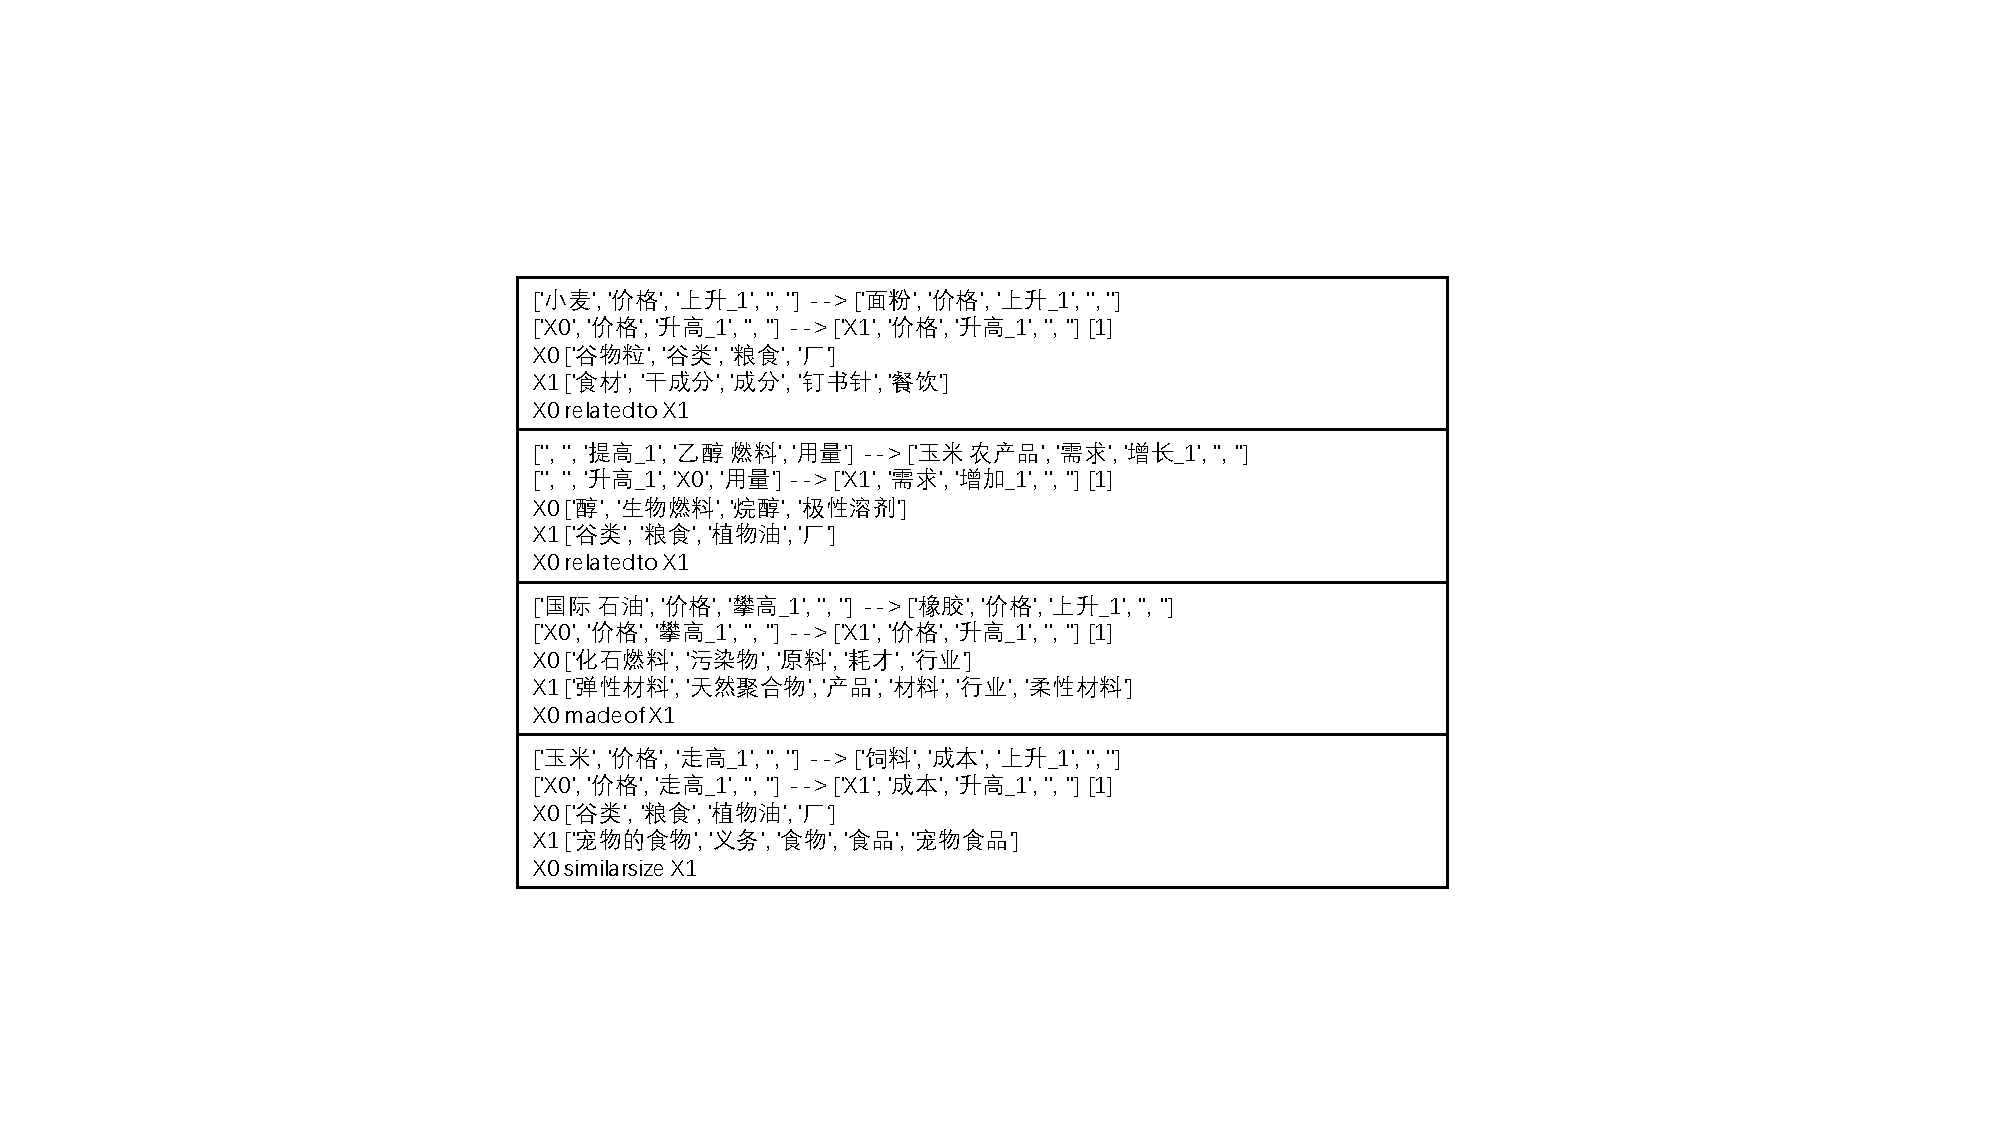
\includegraphics[width=0.95\columnwidth]{figures/reasonable_rule_case}
%	\end{center}
%	\caption{Examples of reasonable Rules.}
%	\label{fig:reasonable_rule_case}
%	\end{figure}
\begin{figure}[htbp]
	\centering
	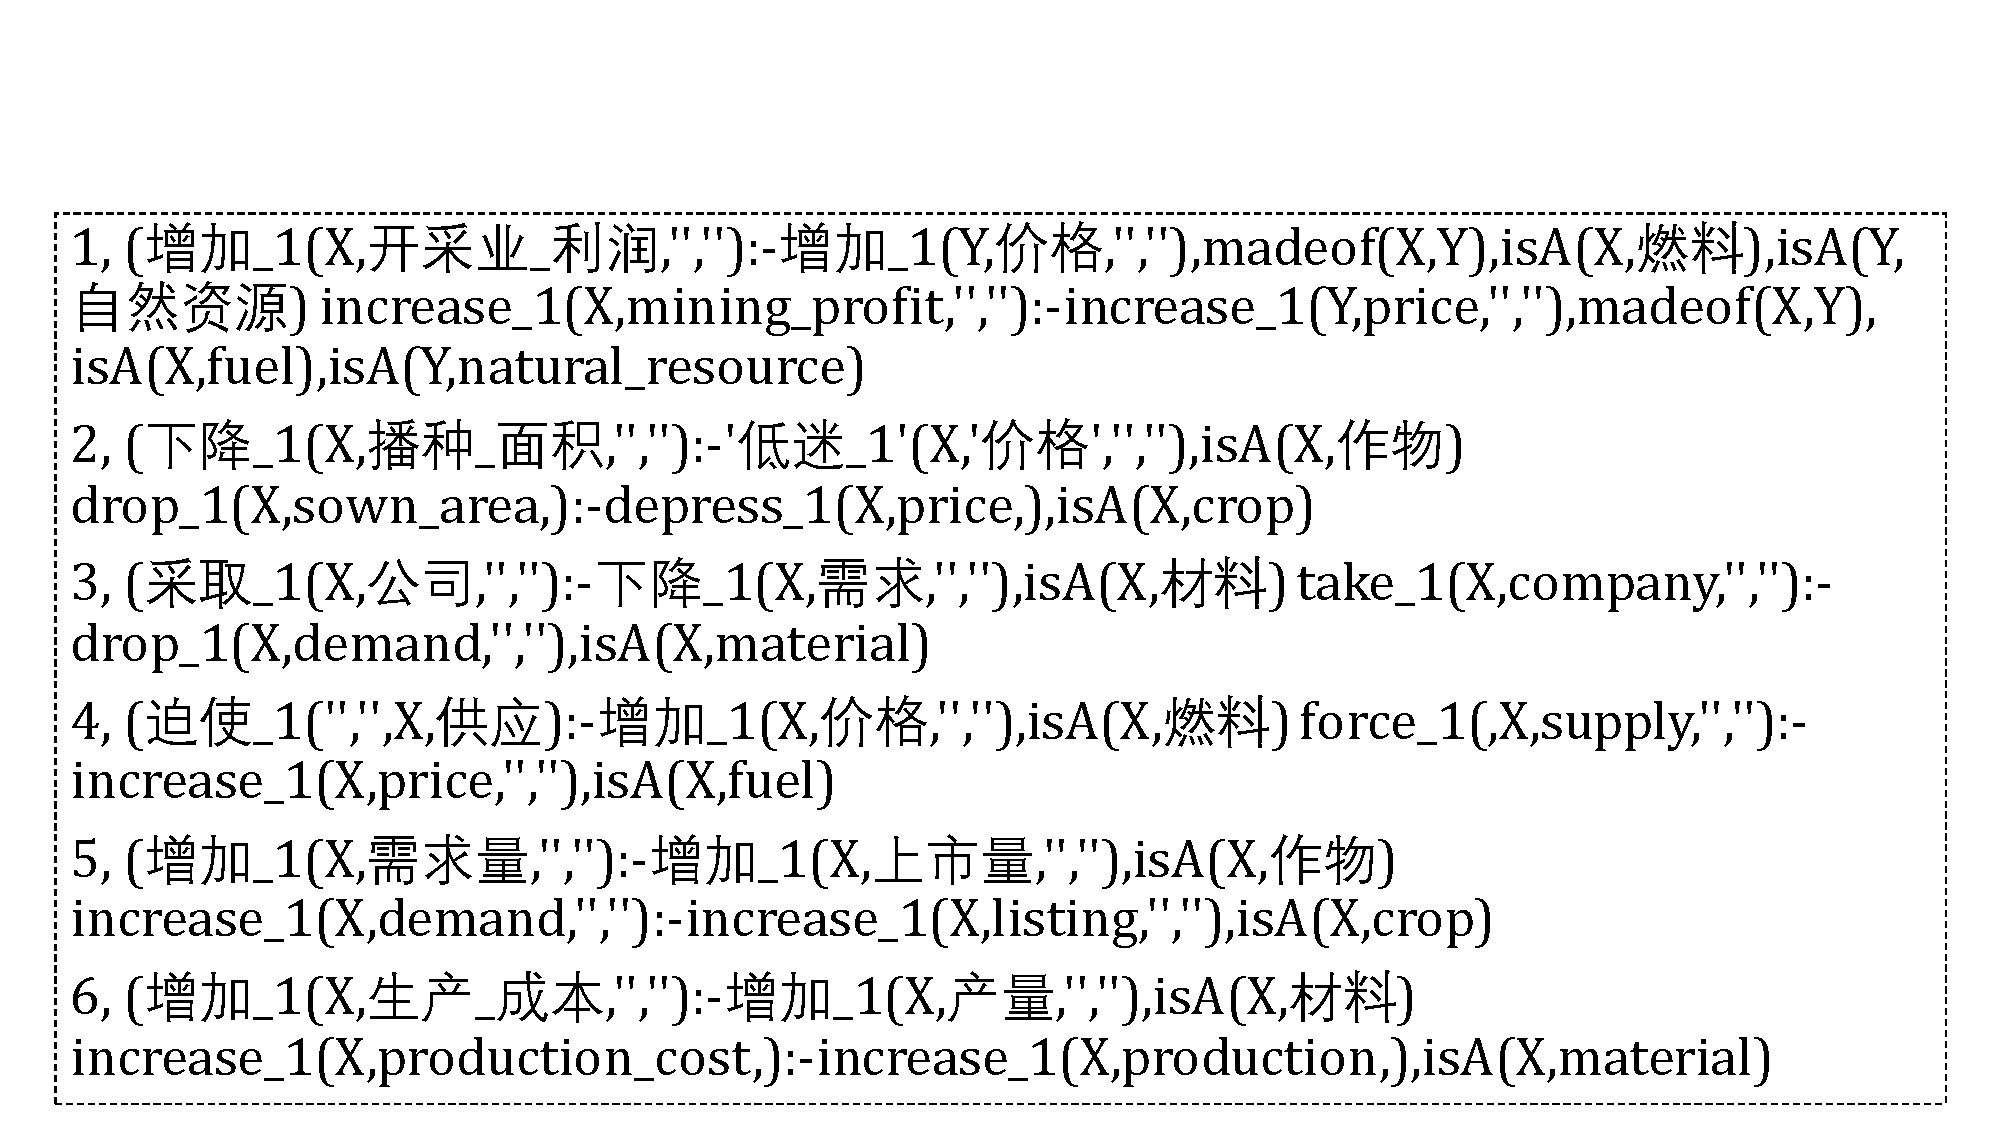
\includegraphics[width=0.95\columnwidth]{figures/rules_case}
	\caption{Examples of Typical Rules}
	\label{fig:rules_case}
\end{figure}
\paragraph{Event Graph}
With these rules, we deduce many rule instances with Prolog and pick out a tiny subgraph about rise and fall events, in Figure\ref{fig:rule_instantiation_graph}, to show the power of the rules. 
	
\begin{figure}[htbp]
\begin{center}
	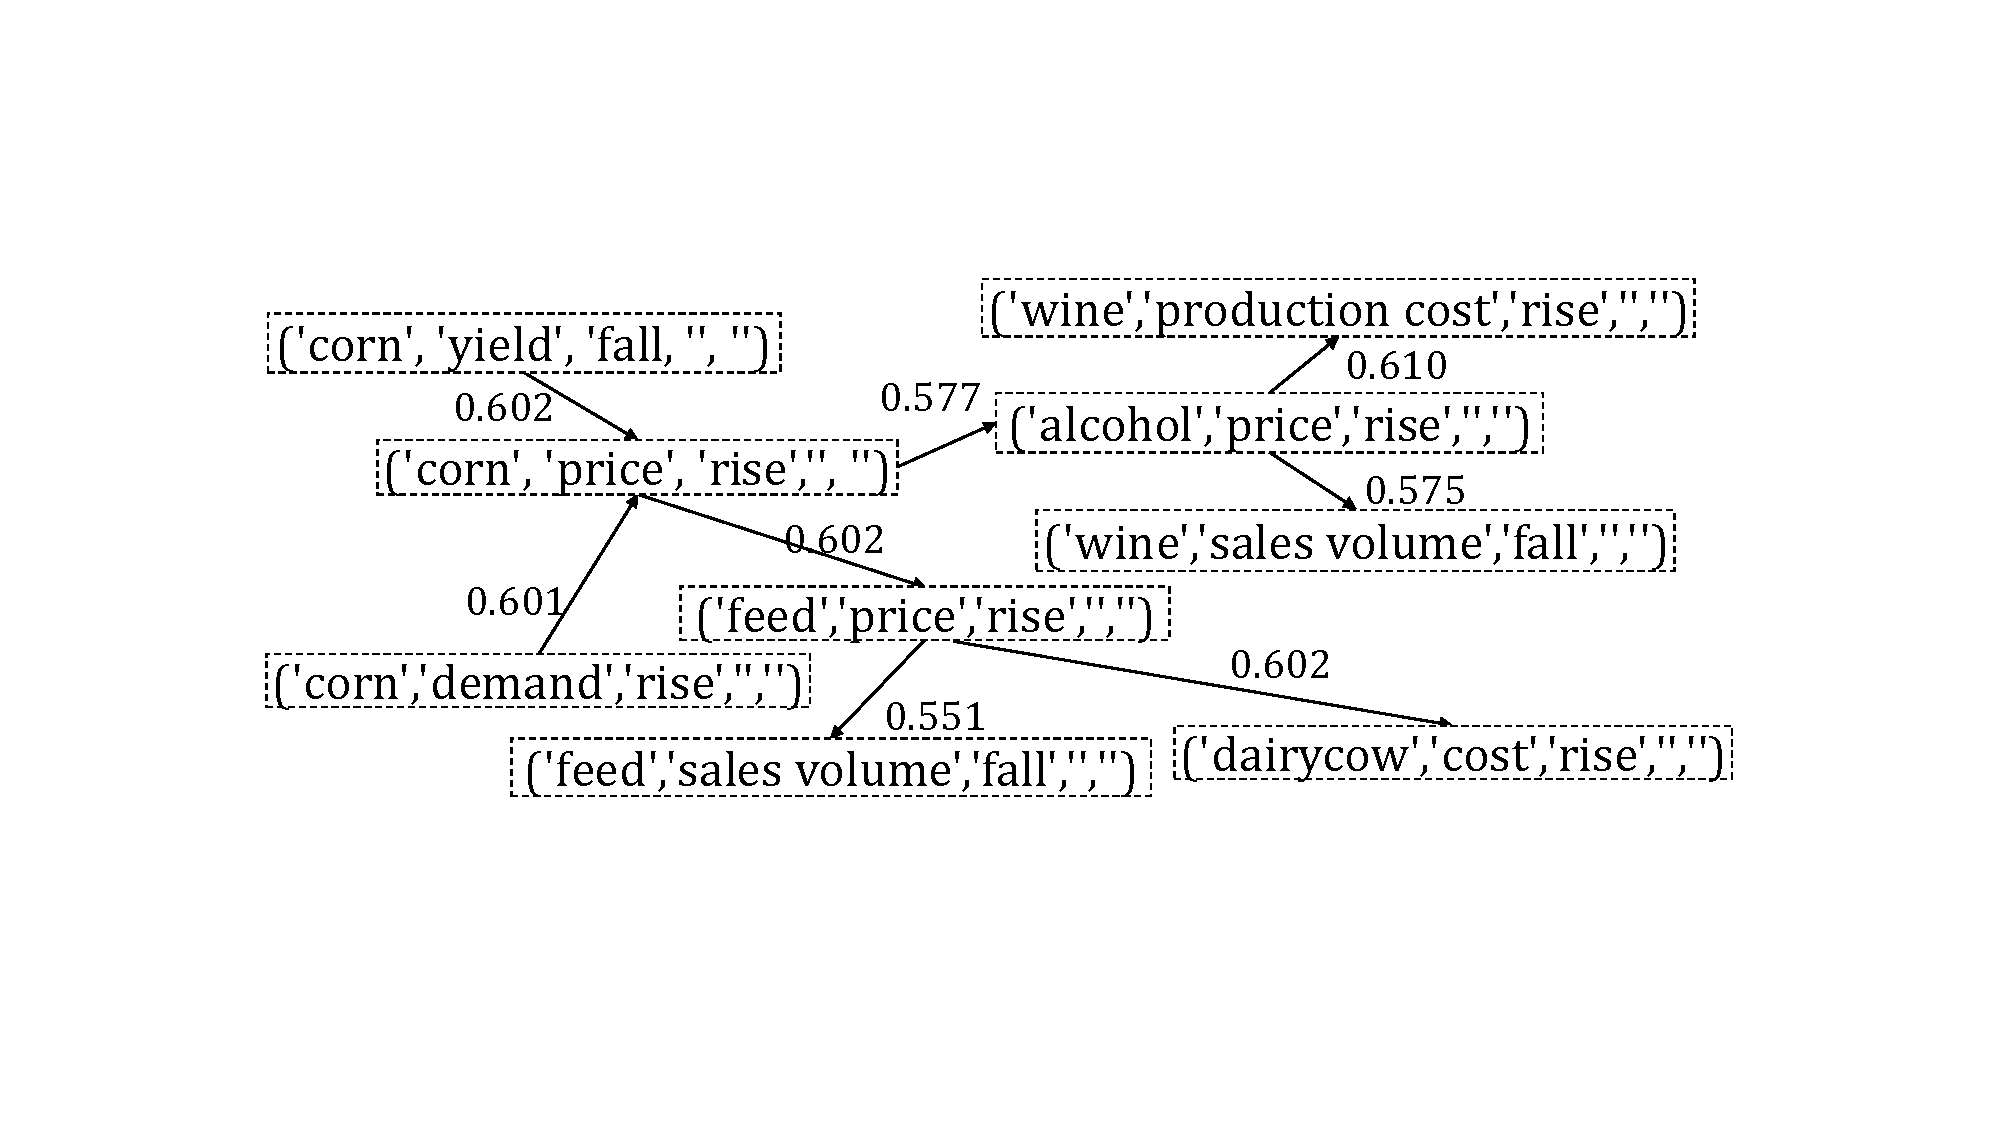
\includegraphics[width=0.9\columnwidth]{figures/instantiation_graph}
\end{center}
\caption{Rule Deduction. As space is limited, we only show the English version and omit the rules used in the reasoning process.}
\label{fig:rule_instantiation_graph}
\end{figure}

\subsection{Comparison with existing Knowledge Bases}
We compare our rules with causal part of other knowledge bases in various aspects in Table \ref{tab:comparison_rule_with_kbs}. We can see our causal knowledge representation is more expressive and informative, and the automatic knowledge acquisition is very convenient.
\begin{table*}[htbp]
\centering
%\begin{tabularx}{\columnwidth}{|c|c|c|c|}\hline
	\begin{tabular}{|c|c|c|c|c|c|c|c|}\hline
	\textbf{Name}&\textbf{Number}&\textbf{Domain}&\textbf{Unit}&\textbf{Data Structure}&\textbf{Information}&\textbf{Source}&\textbf{Precision}\\ \hline
	CausalNet&\textbf{62,675,002}&\textbf{Open}&word&(-)&rich&\textbf{automatic}&-\\
	\multicolumn{8}{|c|}{(`drink',`accident',36)}\\\hline
	ConceptNet &89,416&\textbf{Open}&short text&unstructured&rich&crowdsourcing&\textbf{100\%}\\
	\multicolumn{8}{|c|}{(`smoking',`/r/Causes',`cancer')}\\\hline
	FrameNet&59&\textbf{Open}&frame&\textbf{structured}&richer&crowdsourcing&\textbf{100\%}\\
	\multicolumn{8}{|c|}{Killing(Killer,Place,Means,Victim,Instrument),CausativeOf,Death(Protagonist,Place,Manner,Time)}\\\hline
	ATOMIC&568,312&\textbf{Open}&\textbf{logic event}&semi-structured&much richer&crowdsourcing&86.2\%\\
	\multicolumn{8}{|c|}{If ``PersonX pays PersonY a compliment", Then ``PersonY will smile"}\\\hline
	Ours&50,000&Finance&\textbf{logic event}&\textbf{structured}&\textbf{richest}&\textbf{automatic}&32.5\%\\ 
%			Deductive Rule Instance&\TD{??}\\ 
%	\multicolumn{8}{|c|}{See above rule example in Figure\ref{fig:rules_case}}\\\hline
\multicolumn{8}{|c|}{(Z,`price',`rise',`',`'):-(`',X,`suffer',Y,`attack'),isA(X,`country'),isA(Y,`disaster'),isA(Z,`metal'),atLocation(Z,X) conf:0.842}\\\hline	
	\end{tabular}
%\end{tabularx}  \cite{sap2018atomic}
\caption{Comparison with existing knowledge bases}
\label{tab:comparison_rule_with_kbs}
\end{table*}



%\begin{table}[htbp]
%	\caption{Rule Instance \& Rule}
%	\begin{center}
%	\begin{tabular}{|r|l|}\hline
%		\multicolumn{1}{|c|}{Name}                  & \multicolumn{1}{c|}{Number} \\\hline
%		\multicolumn{1}{|c|}{Rule Instances}        & \multicolumn{1}{c|}{7835403} \\ \hline
%		\multicolumn{1}{|c|}{Rules}                 & \multicolumn{1}{c|}{69036}  \\ \hline
%		\multicolumn{1}{|c|}{more than on relation} & \multicolumn{1}{c|}{2499(3.6\%)}\\
%		\multicolumn{1}{|c|}{only one relation}     & \multicolumn{1}{c|}{66539(96.4\%)} \\
%		\hline
%		==                                          & 56449(84.8\%)                      \\
%		madeof                                      & 5659(8.5\%)                        \\
%		atlocation                                  & 1835(2.76\%)                       \\
%		partof                                      & 1061(1.59\%)                       \\
%		usedfor                                     & 954(1.43\%)                        \\
%		hasa                                        & 511(0.768\%)                       \\
%		derivedfrom                                 & 38(0.0571\%)                       \\
%		hasproperty                                 & 20(0.0301\%)                       \\
%		createdby                                   & 12(0.018\%)                        \\ \hline
%	\end{tabular}
%	\label{tab:rule_statistics}
%\end{center}
%\end{table}
	%Rule Instances & 1817014(4337755)\\
	%Candidate Rules & 86218(201359)\\
	%Rule & 18348(42246)\\

\subsection{Ablation Study}
In this section, we explore the contributions of the various components of our rule learning framework.
\paragraph{Causal patterns statistic} The matched sentences distribution over 3 groups of patterns is shown in Table \ref{tab:pattern_statistics}. All patterns in one group have different causal cue words literally but the same meaning. It shows the third pattern group is more rigorous than the first two groups but has lower usage. Probably because more logical thinking is needed when editing news using more rigorous patterns.

%		\begin{table}[htbp]
%		\caption{Causal patterns. A is a cause tokens span, and B is an effect tokens span. Word '因为' represents a group works like '由于,'是因为','因为','缘于','归因于','原因是','起因','鉴于', and word '所以' represents a group of words like '所以','因而','因此','故此','故而','因故','导致','招致','以致','引致','诱致','致使','造成','使得','从而','从而使','于是','为此'}
%		\begin{center}
%			\begin{tabular}{|c|c|} \hline
%				\textbf{Pattern}& \textbf{Priority}\\ \hline
%				因为 A, 所以B&1\\ \hline
%				A,所以 B&2\\ \hline
%				因为 A,B&3\\ \hline
%			\end{tabular}
%			\label{tab:causal_pattern}
%		\end{center}
%	\end{table}	
	
\begin{table}[htbp]
	\centering
	\begin{tabular}{|c|c|c|c|} \hline
		\textbf{Pattern template}& \textbf{Priority}&\textbf{Number}& \textbf{Rate}\\	\hline 
		因为 A,B&1&2000242&48.32\% \\ \hline 
		A,所以 B&2&1530311&36.96\% \\ \hline 
		因为 A, 所以B&3&576851&14.72\% \\	\hline
	\end{tabular}
	\caption{Number of sentences extracted by causal patterns. A is a cause span and B is an effect span. Word `因为' represents a group works like 由于,是因为,因为,缘于,归因于,原因是,鉴于, and word `所以' represents a group of words like 所以,因而,因此,故而,因故,导致,招致,以致,引致,诱致,致使,造成,使得,从而使,于是,为此}
	\label{tab:pattern_statistics}
\end{table}	
\paragraph{External Knowledge Bases}
The following is some statistics of external knowledge bases used in the rule learning framework. The size of the lexicon is 12,624, obtained from `Industrial classification for national economic activities'\footnote{\url{ http://www.stats.gov.cn/Tjsj/tjbz/hyflbz/}}, which determines which event role in the rule instance can be generalized. 
To our knowledge, most existing Chinese taxonomic knowledge bases, such as CN-Probase\cite{Xu2017}, zhishi.me\cite{Niu2011}, are constructed from online-encyclopedia, which suffer that the concepts inside are far less than Probase and they have no probabilistic character. So we translate Probase to get 11,292,493 Chinese `IsA' pairs.
To our knowledge, there exists no large-scale Chinese commonsense knowledge base, so we translate the English part of ConceptNet and merge the Chinese part to get 2,085,681 Chinese triples.
We randomly sample 500 items from translated Probase and ConceptNet, respectively, and the accuracies after the human evaluation are \textbf{87.8\%}(close to the accuracy of original Probase 92.6\%) and \textbf{91.6\%}.

%\begin{table}[htbp]
%	\centering
%	\begin{tabular}{|c|c|}\hline
%		\textbf{Name}&\textbf{Number}\\ \hline
%		Lexicon&12624\\ \hline
%		Translated Probase &11,292,493(87.8\%)\\ \hline
%		Translated ConceptNet&2,085,681(91.6\%)\\ \hline
%	\end{tabular}
%	\caption{External Knowledge Bases}
%	\label{tab:knowledge_base_statistics}
%\end{table}

%After translation, the number of Chinese IsA pairs is 11,292,493. The number of Chinese commonsense triples is 2,085,681. We both randomly sample 500 items from them, and the accuracy after human evaluation are 0.878 and 0.916 respectively.
%The accuracy of original Probase is 0.926. 
%The number of total Chinese IsA pairs are 11,292,493 which contain concept-instance pairs and concept-subconcept pairs, the. The number of Chinese concepts is 81082 concluding concepts and subconcepts. The number of instances is 158693. The number of Chinese commonsense pairs is 7316977.
%\subsection{External Factual Knowledge Bases}

%From above rule instance extraction submodule, we scan get a rule instances repository. With such huge specific rule instances, we hope to further discover the powerful knowledge hidden in these rule instances. 

%so we generalize such a large amount of rule instances with a more general form. As discussed in Section \ref{sec:intro}, we need to build such a knowledge base. Taxonomy and common sense are two major kinds of knowledge in such knowledge base.
%In our framework, we need to rely on the external Chinese knowledge bases, Chinese Probase and Chinese Conceptnet, to generalize rule instances and add constraints. Most existing Chinese taxonomy knowledge is constructed from online-encyclopedia, such as CN-Probase\cite{Xu2017}. They usually focus more on named entity such as famous movie stars, singer stars, while we care more about the concrete things existed in life such as corn, steel, alcohol and so on.  In addition, they have no probabilistic character. Translation is an effective and efficient approach, we choose to translate Probase, which is a probabilistic taxonomic knowledge base.
%To our knowledge, there exists no large-scale Chinese commonsense knowledge base, so we translate the English part of ConceptNet5 into Chinese and combine the Chinese part.

%	 which is special for this, But it is only for English. We have investigated the CN-Probase\cite{xu2017cn}, but It even can't find the concept of common entities like '中国/China', '橡胶/rubber' and it also limits the usage frequency. So we collect the items from Probase, the items with 'IsA' relation in ConceptNet5\cite{speer2013conceptnet}, Webbrain\cite{chen2016webbrain}. Then, we fuse them together, Then, translate them into Chinese with google translator. to reduce the translate error, we put more context into the translator as more as possible, for example we put 'fruit such as apple, banana', Then we can get the translated result of IsA(apple,fruit), IsA(banana, fruit) together, which can make word sense of 'apple' to be translated near the fruit not company.  
%	\subsubsection{Chinese Commonsense knowledge base.}
%	, consisting of 47, 3, 25 relations respectively. Some of them are duplicative and some are useless for us. So we select specific number useful relations and we also design some patterns to extract some relations from Chinese wiki. 
%	relattions between arguments are used in rule specialization submodule to make rules reasonable. There exist many commonsense knowledge bases such as ConceptNet5, WebBrain, WebChild.  The numbers of the relations in these knowledge bases are limited. And some relations are equivalent among different knowledge bases, such as '/r/RelateTo' in ConceptNet is equivalent to 'relateto' in WebBrain. So we normalize all the relations names literally.
% Meanwhile, many pairs of arguments have more than one relations which are  duplicated semantically. For example, (sweet corn, corn) has the relations 'relatedto' and 'partof', obviously, 'partof' consists of 'relatedto' semantically. So we hope to remove the semantic reduplication relations. which means we need find the semantic containment relations among these relations.
%Algorithm \ref{alg:alg1} shows the Relations Containment algorithm we proposed. It firstly counts each relation and its corresponding arguments pairs. Then, compare the every two correlated relations, and record their containment relation. Last, enumerate all relations in each pair of arguments, remove the relation which is not contained in other relations existed in this pair of arguments.
%When fusing these knowledge bases, we regard arguments from different knowledge bases which have the same literal name as the same arguments.
%	from structured information to knowledge which is close to intelligence
%The goal of rule acquisition is to learn first-order logic rule from huge number of rule instances with the support of external factual knowledge, shown in the Figure \ref{fig:overview}'s middle part.
%with the knowledge base, now, we can generalize the rule instances extracted from rule instances extraction submodule into candidate rules to represent more general knowledge. For example, we hopefully generalize from each cluster of rule instances to one candidate rule. For example, given two rule instances in one cluster, ('国际 石油', '价格', '攀高@攀高', '', '') $->$ ('橡胶', '价格', '上升@升高', '', '') and ('国际 柴油', '价格', '攀高@攀高', '', '') $->$ ('橡胶', '价格', '上升@升高', '', ''), the generalized candidate rule would be('X0', '价格', '攀高', '', '') $->$ ('X1', '价格', '升高', '', '') where 'X0' IsA' 化石燃料','原料' and  'X1' IsA '弹性材料' '天然聚合物'.


%\begin{table}[htbp]
%\centering
%		\begin{tabular}{|c|c|}\hline
%			\textbf{Name}&\textbf{Number}\\ \hline
%			Lexicon&12624\\ \hline
%			Concepts &18281\\	
%			IsA pairs &123547\\
%			Concept-subconcept pairs&18753\\
%			Concept-instance pairs&104794\\\hline
%			Commonsense Pairs&32593\\ 
%			Commonsense Relations&10\\ \hline
%		\end{tabular}
%		\caption{Knowledge Base}
%		\label{tab:knowledge_base_statistics}
%\end{table}
\paragraph{Open Event Extraction}
%	TextRunner/WOE,ReVerb,Ollie,ClausIE,SRL/AMR parsing/frame-semantic parsing,NestIE 
Since our event structure scheme is plain and straightforward, we choose the reliable Stanford CoreNLP tool to extract the rule instances.
%	rule instance  97/200(48.5\%)& 21/200(10.5\%) & 82/200(41.0\%) \\ \hline
The number of rule instances extracted after rule instance distilling submodule is 7,835,403. Since most of them are discarded in the learning process, the number of rule instances really used for rule induction is 78,098 with an accuracy of \textbf{48.5\%} (we also sample 200 rule instances and manually evaluate them).

%\textit{To sum up}, our framework is a pipeline, in which rule instance extraction achieve 48.5\%, ConceptNet5 translation achieve 91.6\% and Probase translation achieves 87.8\%, So teh rule finally can achieve 39.0\%(48.5\%*91.6\%*87.8\%) maximumly, which is close to the evaluation of the final rules. 

%\textbf{\textit{To sum up}}, 
%our framework is a pipeline, in which the accuracy of rule instance extraction is 48.5\%, the accuracy of ConceptNet5 translation is 91.6\%, and the accuracy of Probase translation is 87.8\%. 
\textbf{\textit{To sum up}}, our framework is a pipeline undergoing rule instance extraction(accuracy 48.5\%), constrain relations addition(accuracy of ConceptNet 91.6\%), and rule induction(accuracy of Probase 87.8\%).
Thus, the accuracy can only reach \textbf{39.0\%} (48.5\%*91.6\%*87.8\%) at the maximum, which is close to our evaluation(32.5\%) of the final rules.

%	\subsubsection{Rule Acquisition}
%	\begin{table}[]
%		\centering
%		\begin{tabular}{lll}
%			& rule number  & qualitity       \\
%			no Coneptnet / only one relation    & 66539/96.4\% & informative     \\
%			Conceptnet / more than one relation & 2499/3.6\%   & more infrmative
%		\end{tabular}
%		\caption{Relation Number}
%	\end{table}

%	\begin{table}[]
%		\caption{Event Connection}
%		\begin{center}
%		\begin{tabular}{lll}
%			==         & 60475 & 84.4\%  \\
%			madeof     & 6161  & 8.6\%   \\
%			atlocation & 2104  & 2.94\%  \\
%			partof     & 1152  & 1.61\%  \\
%			usedfor    & 1072  & 1.5\%   \\
%			others     & 674   & 0.941\%
%		\end{tabular}
%		\end{center}
%	\end{table}
\subsection{Application: Futures Price Prediction}
%\paragraph{Reasoning with Uncertainty}
\begin{figure}[htbp]
	\begin{center}
		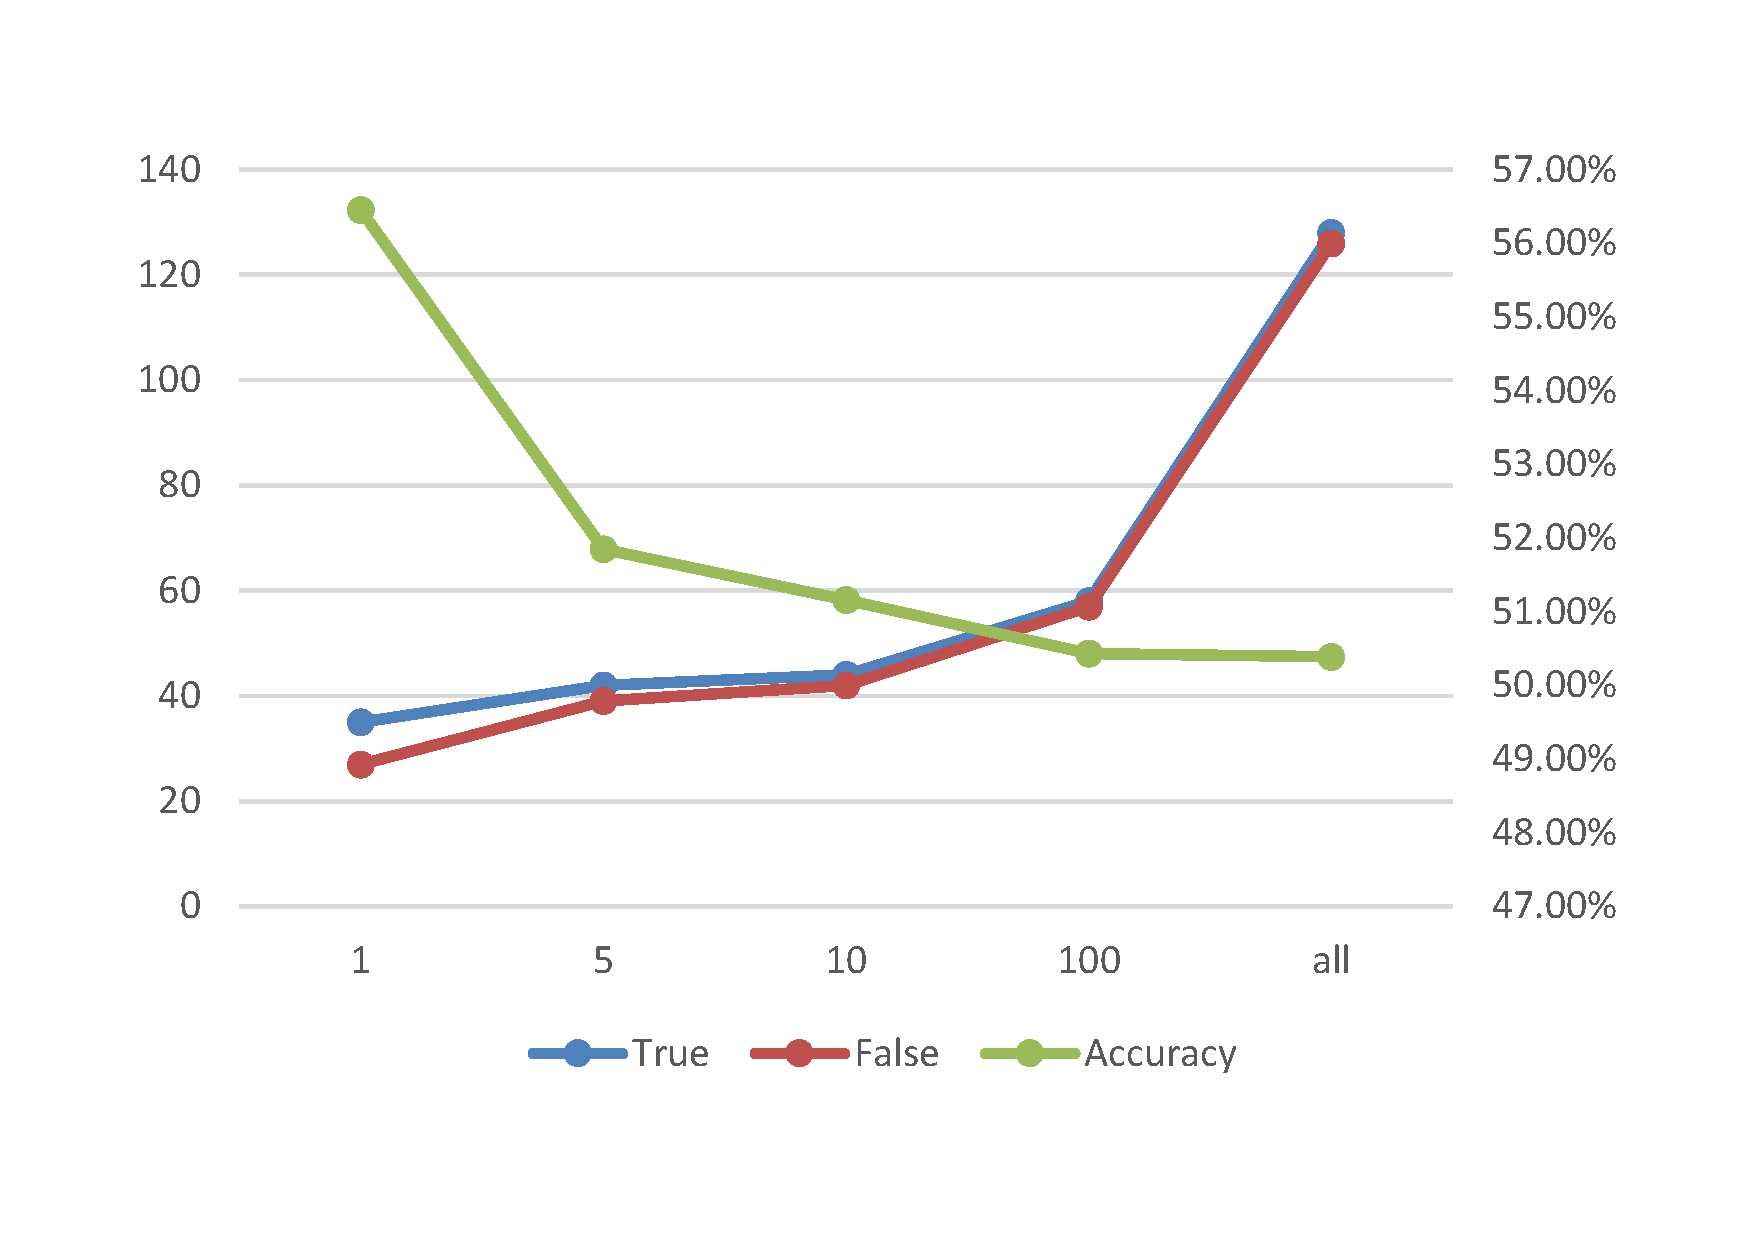
\includegraphics[width=0.9\columnwidth]{figures/rule_futures_prediction}
	\end{center}
	\caption{Futures Price Prediction.}
	\label{fig:futures_price_prediction}
\end{figure}
We choose futures price prediction because the futures are common and concrete things existed in ConceptNet and Probase, such as corn, oil, etc.
%\cite{Ding} is the state-of-the-art stock prediction model(EB\_CNN). We follow similar experimental settings. 
We follow similar experimental settings in \cite{Ding}.
From 2018/1/1 to 2018/11/2, we collect all the headlines and the price change of 15 futures as test data, which include \textbf{851} price change events (The price change of more than 1\% relative to the previous day is an event and we only focus on rise or fall events). 

Baseline models: EB\_CNN model \cite{Ding}, the state of the art model in stock price prediction, uses a deep convolutional neural network to model both short-term and long-term influences of events on stock price movements, and the accuracy of futures prediction is \textbf{54.2\%}. Other models in \cite{Ding}, such as EB\_NN, WB\_CNN, and WB\_NN can achieve \textbf{53.0\%}, \textbf{53.2\%}, and \textbf{53.5\%}, respectively. These accuracies of futures prediction are lower than the accuracies of stock prediction shown in the paper.
It may be because the factors affecting the futures price are far less than the stock price and the futures price is much more stable than the stock price, which makes useful training information about the futures less and further affects the accuracy of the models.

Our approach: For each actual future price change event , we get the news headlines for the previous month before this event. 
For each news headline, we extract the event, use Prolog to reason based on the rules and external knowledge bases, and get the top K inferred events sorted by the confidence.
We may have m*K inferred events for this event, m is the number of events occurred in this month. 
Here, we select the price change events(rise or fall) of the future in this actual future price change event from m*K events and calculate the weighted sum of their confidences(rise event weights 1 and fall event weights -1). If the sum value is positive, we predict this future price as a rise event, otherwise as a fall event. If get no related events changing the future's price, do not make prediction. We compare this prediction with the actual price change to evaluate the reasoning effect. 
Figure \ref{fig:futures_price_prediction} shows the average prediction result. It shows the more predicted events inferred from the Prolog(by increasing K) we use, the lower the prediction accuracy is(from \textbf{56.5\%} to \textbf{50.4\%}), and the more futures events we can predict(from \textbf{62} to \textbf{254}). 

\textbf{\textit{To sum up}}, our rule-based prediction approach can have a higher prediction accuracy (56.45\%) and better interpretation ability with a low recall rate, which is very practical in life.

%\begin{table}[htbp]
%	\caption{Baselines and Proposed Framework}
%	\begin{center}
%		\begin{tabular}{lll}\hline
%			& Acc & MCC \\\hline
%			WB-NN &  0.535 &     \\
%			WB-CNN&  0.532  &     \\
%			EB-NN &  0.530  &     \\
%			EB-CNN&  0.542   &     \\
%			Rule &     &    \\\hline
%		\end{tabular}
%		\label{tab:baselines_and_rule}
%	\end{center}
%\end{table}

\subsection{Downloading and Demo}
The translated Chinese Probase and ConceptNet and learned rules are available at URL.
We built a demo to demonstrate the reasoning process at URL. 
We also developed an application demo of futures prices change triggering that can monitor news from around the world in real time, find the news that may cause futures prices changes, and alert users. Visit URL.
%\section{Related Work}
\paragraph{Clarification Question Generation} The concept of CQ can be naturally raised in a dialogue system where the speech recognition results tend to be erroneous so that we raise CQs for sanity check \citep{stoyanchev2014towards}, or the intents for a task is incomplete or ambiguous in a first short utterance and further CQs are needed to fill in the slots \citep{dhole2020resolving}. The concept is then extended to IR to clarify ambiguous queries \citep{aliannejadi2019asking}, and has been successfully put into practice \citep{zamani2020generating}. Other application areas including KBQA \citep{xu2019asking} and open-domain dialogue systems \citep{aliannejadi2020convai3}. CQGen can also be applied to help refine posts on websites like StackExchange \citep{Kumar_2020} and Amazon \citep{rao2019answer}. In this context, our work closely follows the research line of \citep{rao2018learning, rao2019answer, cao2019controlling}. \citet{rao2018learning} first adopted a retrieval-then-rank approach. They \citep{rao2019answer} then proposed a generation approach to train the model to maximize the utility of the hypothetical answer for the questions with GAN, to better promote specificity. \citet{cao2019controlling} propose to control the specificity by training on data with explicit indicator of specificity, but it requires additional specificity annotation. Towards the similar specificity goal, we adopted a different keyword-based approach. They also assume generating one question per context, which we claim is not sufficient to cover various possible information needs, and thus propose the task of the diverse CQGen.

\paragraph{Diverse Generation} The demand for diverse generation exists in many other fields~\cite{vijayakumar2018diverse, LiangZ18code, shen2019mixture}, and we've drawn inspirations from these literatures. For image captioning, we may use multiple descriptions for different focusing points of a scene. \textit{Diverse Beam Search} \citep{vijayakumar2018diverse} was proposed to broaden the searching space to catch such diversity by dividing groups in decoding and imposing repetition penalty between them. For machine translation, a context can be translated with different styles. \citet{shen2019mixture} thus proposed \textit{Mixture of Expert} models including hMup to reflect various styles with a discrete latent variable (\textit{expert}). And here for CQGen, diversity is required to cover various potentially missing aspects, so we come up with the idea to use keywords as a controlling variable like \textit{expert} to promote diversity.


\section{Conclusion}

In this paper, we incorporated the idea of Cookie Theft picture description task into the evaluation of the high-level cognitive abilities of LVLMs and designed a novel evaluation benchmark called CogBench.
% Images in CogBench are of high quality and require more cognitive reasonings to understand, which makes it different from existing image datasets.
The images in CogBench are of high quality and demand more complex cognitive reasoning for interpretation, setting it apart from existing image datasets.
% It consists of a image description task and a VQA task.
Experiments show that there is still a large gap between the cognitive abilities of LVLMs and human beings, indicating CogBench is a challenging benchmark.

% In the future



\bibliographystyle{acl_natbib}
\bibliography{acl2018}
\end{document}
